\chapter{Feasibility of Learning}\label{Sec:Feasibility of Learning}

No practical amount of data can distinguish between two distributions, thus instances of GBS can not be proven to come from GESIS. However, machine learning allows to infer the conditional probability of \textit{'GBS participant is representative'} given the survey data within a probabilistic framework. A well-defined learning problem involves a number of design choices, including selecting the target function to be learned, a representation for this target function, and an algorithm to learn from the source of training experience \cite{tom}. This paper defines key terminology of the theoretical aspects of survey analysis and machine learning. The MRS algorithm is then formulated as positive-unlabeled learning problem in addition to traditional machine learning.

\section{Sampling Bias}

Variables considered in the GBS study must accurately reflect the populations characteristics. That is, every element of the population has a known non-zero chance of being selected. This includes people whether or not they choose to take part in the survey. Results can then be used to make estimates for not only the sample itself but also the target population. A sampling method is called biased if it systematically favors some people over others, e.g. by oversampling people with strong opinions and undersampling people who do not care much about the topic of the survey \cite{west}.

Sampling bias is often referred to as selection bias or sample selection bias. I will stick to the more descriptive term sampling bias. It underlines the fact that the bias arises in how the data was sampled. Also, the use of the term becomes less ambiguous, because there exists another notion of selection bias in the context of model selection. This type of bias is usually referred to as bad generalization, where the performance of the selected hypothesis is overly optimistic \cite{yaser}.

\section{The Problem of Overfitting}

Overfitting stands out as one of the biggest challenges for machine learning. It is not exclusive to machine learning but rather a fundamental problem across science and is at the very heart of the dangers of statistical inference. Hypothesis \(h\) in \(H\) overfits training data if there exists an alternative hypothesis \(\bar{h}\) in \(H\) such that \(errorTrain(h) < errorTrain(\bar{h})\) and \(errorD(h) > errorD(\bar{h})\), where \(errorTrain(h):=\) error of hypothesis \(h\) over training data and \(errorD(h):=\) error over entire distribution \(D\) of data. A hypothesis overfits the training examples if some other hypothesis that fits the training examples less well actually performs better over the entire distribution of instances \cite{yaser}.

When overfitting occurs, the learned hypothesis is very good at calculating the answers for the given data, but much less so for new instances it encounters. In a sense, the machine learning algorithm has become fixated on unimportant features of the training data overlooking the big picture. It often occurs when the algorithm has too many options to play with in designing its mappings, an approximation of the target function. The freedom to tune parameters and add complexity until it exactly matches the training data, rather than looking for large, systematic patterns leads to high variance \cite{yaser}.

The expected prediction error at any given data point \(x_0\), the generalization error, can be decomposed as follows \cite{ian}: 
\begin{align*}
Err(x_o) &= \EX[(Y - \bar{f}(x_0))^2 \mid X = x_0] \\
& =  \sigma^2_\epsilon + [\EX\bar{f}(x_0) - f(x_0)]^2 + \EX[\bar{f}(x_0) - \EX\bar{f}(x_0)]^2\\
& =  \sigma^2_\epsilon + Bias^2(\bar{f}(x_0)) + Var(\bar{f}(x_0)) \\
& = Irreducible Error + Bias^2 + Variance
\end{align*}

The bias and variance terms make up the error of \(\bar{f}(x_0)\) in estimating \(f(x_0)\). The bias component is the squared difference between the true mean \(f(x_0)\) and the expected value of the estimate \([\EX\bar{f}(x_0) - f(x_0)]^2\), where the expectation averages the randomness in the training data. The variance term refers to the amount by which the estimate of the target function would change if it was estimated using a different training data set. Ideally the estimate for the underlying pattern should not vary too much between training sets. More generally, as the model complexity is increased, the variance tends to increase and the squared bias tends to decrease. The opposite behavior occurs as the model complexity is decreased. The first term in this expression is the irreducible error, a combination of stochastic and deterministic noise. More precisely, stochastic noise are fluctuations or measurement errors that can not be modelled. Re-measuring \(y_n\) changes this component. Deterministic noise is the part of the target function that can not be represented. Changing \(H\) changes this component. With a single dataset \(D\) and fixed \(H\) it is impossible to distinguish \cite{yaser}.  

\section{Discriminative Learning} 

With the definitions above, a model is not necessarily overfitting because of poor generalization performance. It simply gets much more complicated to analyse sources of error in a covariate-shift setting. To evaluate the actual performance of a model, the given data samples must be split properly.

Several approaches exist to deal with positive and unlabeled data. The most straightforward one is to assume that all the unlabeled data are negative and simply apply standard machine learning techniques (Neelakantan, Roth, and McCallum 2015).

The error rate on the training data, the resubstitution error, as turned out to be overly optimistic, is not a good indicator of performance on future data. The holdout estimate can be made more reliable by repeating the process with different subsamples. The error rates on the different iterations are averaged to yield an overall error rate.

There is almost always not enough data available to partition it into separate training and test sets without losing significant modelling or testing capability. In these cases, a fair way to properly estimate model prediction performance is to use cross-validation as a powerful general technique \cite{ian}.

The intuition for these results comesfrom the fact that in many practical situations, the posteriordistributions in traditional and non-traditional setting pro-vide the same optimal ranking of data points on a given testsample (Jain et al. 2016; Jain, White, and Radivojac 2016).

\begin{figure}[ht]
	\begin{center}
		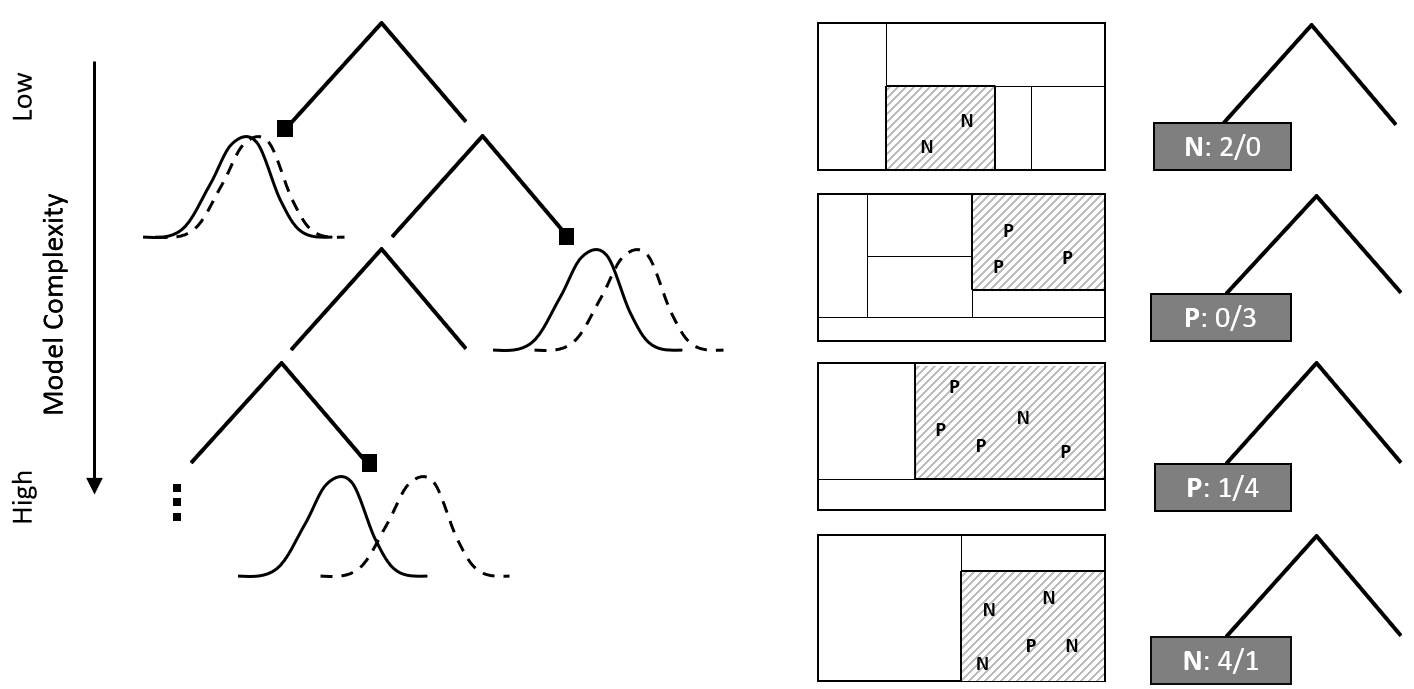
\includegraphics[scale=0.40,angle=0]{fig/tree3}
		\label{project}
		\caption{.}
	\end{center}
\end{figure}

\section{Learning from Positive and Unlabeled Data}

To further reduce the variance of the error estimate, each class is sampled with approximately equal proportions in both datasets, a technique called stratification. 

We have shown the effect of resampling contaminated sets and provided some basic insight into the mechanics of bagging. We will now link these two elements to justify bagging approaches in the context of contaminated training sets. Its usefulness can be considered by both the variance reduction argument of Bauer and Kohavi [4] and equalizing the influence of training points as described by Grandvalet [24]. Variance reduction. Resampling a contaminated set yields different levels of contamination in the resamples as explained in Section 3.1. Varying the contamination between base model training sets induces variability between base models without increasing bias. This observation enables us to create a diverse set of base models by resampling both P and U. The variance reduction of bagging is an excellent mechanism to exploit the variability of base models based on resampling [4, 10]. In the context of RESVM, a tradeoff takes place between increased variability (by training on smaller resamples, see Figure 1) and base models with increased stability (larger training sets for the SVM models).

PU learning is a semi-supervised technique that does not make the simplifying assumption of GBS instances being negative. Instead, a one-class classifier is trained on GESIS only. [...] This can result in even better assessment. [Read Literature] - Imporance weighted cross validation and pu learning with proper assessment. State-of-the-art techniques in positive-unlabeled learningtackle this problem by treating the unlabeled sample as neg-atives and training a classifier to distinguish between la-beled (positive) and unlabeled examples. Surprisingly,for a variety of performance criteria, non-traditional classi-fiers achieve similar performance under traditional evalua-tion as optimal traditional classifiers (Blanchard et al. 2010;Menon et al. 2015). 

\vspace{0.4cm}

\begin{algorithm}[H]
\caption{PU training procedure}\label{alg:alg}
\vspace{0.2cm}
\KwIn{\(P\): set of positive instances (GESIS)}
\myinput{\(U\): set of unlabeled instances (GBS)}
\myinput{\(n_{models}\): number of base models in ensemble}
\myinput{\(n_P\): size of bootstrap sample of \(P\)}
\myinput{\(n_U\): size of bootstrap sample of \(U\)}
\KwResult{Scoring function \(f:U \rightarrow \) $\mathbb{R}$}
Initialize: 
\(f(x) \leftarrow 0\) and 
\(c(x) \leftarrow 0\)\\
\For{t = 1 to \(n_{models}\)}{
\hfill \\
  Draw a bootstrap sample \(P_t\) of size \(n_P\). \\
  Draw a bootstrap sample \(U_t\) of size \(n_U\). \\
  Train classifier \(f_t\) to discriminate \(P_t\) against \(U_t\). \\
  For any \(x \in U \backslash U_t\), update: \\
\(f(x) \leftarrow f(x) + f_t(x),\) \\ 
\(c(x) \leftarrow c(x) + 1\) \\
\vspace{0.2cm}}
Return: \(s(x) = f(x)/c(x)\)
\vspace{0.3cm}
\end{algorithm}

\begin{comment}
\begin{algorithm}[H]
\caption{Transductive bagging PU learning}\label{alg:alg2}
\KwIn{\(P\): set of positive instances (GESIS)}
\myinput{\(U\): set of unlabeled instances (GBS)}
\myinput{\(K_P\): size of bootstrap samples, \(T\): number of base models in ensemble}
\KwResult{Ranking score \(s:U \rightarrow \) $\mathbb{R}$}

\For{t = 1 to \(T\)}{
 Draw a bootstrap sample \(P_t\) of size \(K_P\). \\
 Train classifier \(f_t\) to discriminate \(P_t\) against \(U\). \\
 For any \(x \in U \backslash U_t\), update:
\[f(x) \leftarrow f(x) + f_t(x),\]
\[n(x) \leftarrow n(x) + 1\]
}
Return \[s(x) = f(x)/n(x)\]

\end{algorithm} 
\end {comment}

The most extensively studied and widely used performance evaluation in binary classification involves estimating the Receiver Operating Characteristic (ROC) curve. The ROC curve plots the true positive rate (recall) of a classifier as a function of its false positive rate (Fawcett 2006) over a range of decision thresholds. Furthermore, AUC has a meaningful probabilistic interpretation that is used to  the ability of the classifier to separate classesand is often used to rank classifiers (Hanley and McNeil1982). the widely-accepted evaluation approaches us-ing ROC curves are insensitive to the variation ofraw prediction scores unless they affect the ranking.

Let \(f\) be the true distribution over the input space \(X\) from which unlabeled data is drawn. With distributions \(f_1\) and \(f_0\) of the positive and negative examples, respectively, it follows that
\[f(x) = \alpha f_1(x) + (1-\alpha)f_0(x)\]
with positive class prior \(\alpha \in [0,1], x \in X\).

Consider the binary classification problem from input \(x \in X\) to output \(y \in Y\) (representative: '\(1\)', not representative: '\(0\)'). The learning objective is to discriminate between \(X_p\) drawn according to \(f_1\) and \(X_u\) drawn according to \(f\)  and recover its performance estimate in the traditional setting, i.e. evaluating the decision boundary between positive and negative data.

Recall \(\gamma\), false positive rate \(\eta\) and precision \(\rho\) are defined as: \(\gamma = P[\hat{Y} = 1| Y = 1]\), \(\eta = P[\hat{Y} = 1| Y = 0]\) and \(\rho = P[Y = 1| \hat{Y} = 1]\), where \(\hat{Y}\) is an estimate of the true class label \(Y\). TPR \(\gamma\) can be estimated directly, because \(X_p\) was sampled from \(f_1\), while this does not hold true for \(\eta\) given the absence of samples from \(f_0\). 
\begin{gather*}
\gamma = \e{f_1[h(x)]} = \frac{1}{|X_p|} \sum\nolimits_{x \in X_p} h(x) \\
\hat{\eta}^{pu} = \e{f[h(x)]} = \frac{1}{|X|} \sum\nolimits_{x \in X} h(x)
\end{gather*}

The area under ROC curves \(AUROC^{pu}\) so far could only be estimated for the positive versus unlabeled classification by plotting \(\gamma\) and \(\hat{\eta}^{pu}\). To calculate \(AUC\) from \(AUC^{pu}\), S. Jain et al. (2015) express \(\eta\) in terms of \(\hat{\eta}^{pu}\) and \(alpha\) and provide a full derivation from the probabilistic definition of the AUC with

\[\eta = \frac{\hat{\eta}^{pu} - \alpha \gamma}{1 - \alpha}\] so that

\[AUC = \frac{AUC^{pu} - \frac{\alpha}{2}}{1 - \alpha}\] proving

\[AUC > AUC^{pu} \iff AUC^{pu} > \frac{1}{2}\].